\documentclass[dvipdfmx,autodetect-engine,titlepage]{jsarticle}
\usepackage[dvipdfm]{graphicx}
\usepackage{ascmac}
\usepackage{fancybox}
\usepackage{listings}
\usepackage{plistings}
\usepackage{itembkbx}
\usepackage{amsmath}
\usepackage{url}
\usepackage{graphics}
\usepackage{here}

\lstset{
  basicstyle={\ttfamily},
  identifierstyle={\small},
  commentstyle={\smallitshape},
  keywordstyle={\small\bfseries},
  ndkeywordstyle={\small},
  stringstyle={\small\ttfamily},
  frame={tb},
  breaklines=true,
  columns=[l]{fullflexible},
  numbers=left,
  xrightmargin=0zw,
  xleftmargin=3zw,
  numberstyle={\scriptsize},
  stepnumber=1,
  numbersep=1zw,
  lineskip=-0.5ex
}

\textheight=23cm
\renewcommand{\figurename}{図}
\renewcommand{\tablename}{表}
\newenvironment{code}
{\vspace{0.5zw}\VerbatimEnvironment  \begin{screen} 
\baselineskip=1.0\normalbaselineskip
 \begin{Verbatim}}
{\end{Verbatim}
\baselineskip=\normalbaselineskip
 \end{screen}\vspace{0.5zw}} 

\title{ワイヤレス通信システム(B1)\\
9th Week 相互インピーダンス\\
}
\author{2600200087-2\\Oku Wakana\\奥 若菜}
\date{Jun. 27 2022}

\begin{document}

\maketitle

\section{半波長ダイポールアンテナの相互インピーダンス}
教科書39ページの図3.8のグラフをMATLABを用いて描画した。得られたグラフを図1に、その際のソースコードを下に示す。\\

\begin{figure}[H]
  \centering
  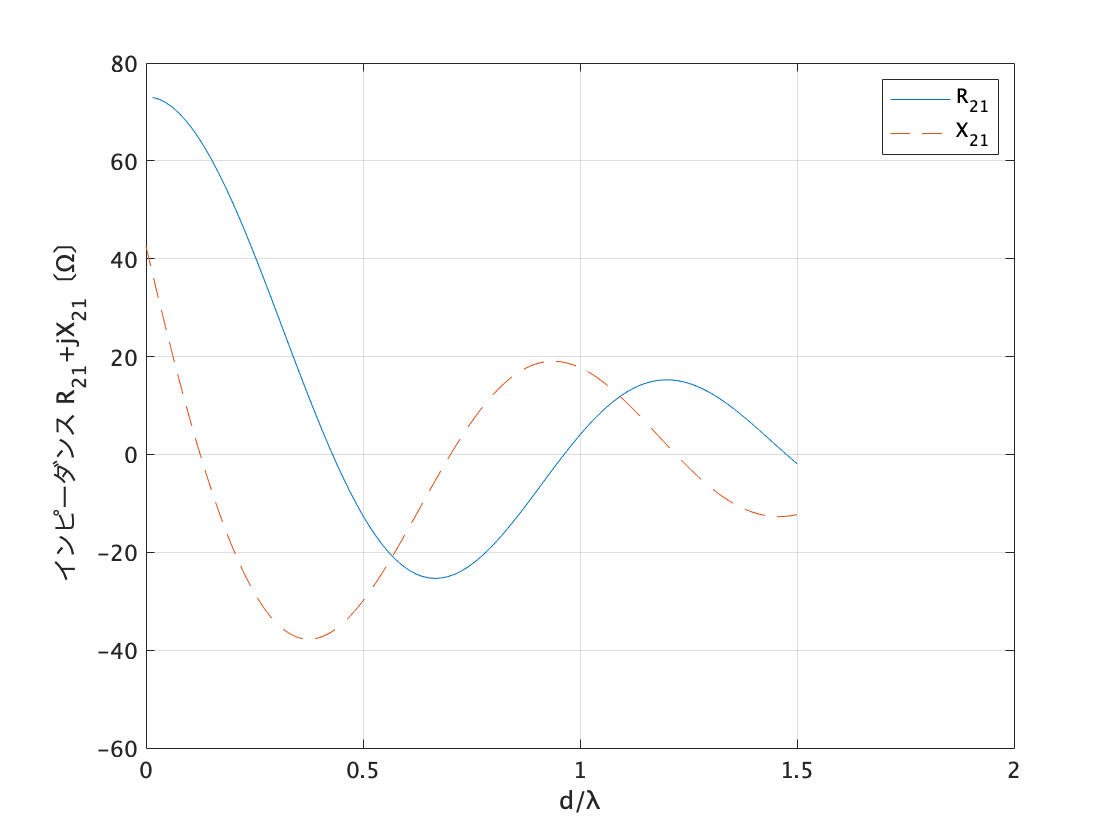
\includegraphics[scale=0.27]{week9_1.png}
  \caption{半波長ダイポールアンテナ間の相互インピーダンス}\label{fig:図1}
\end{figure}
 \\

\begin{lstlisting}[caption=ソースコード,label=1]
figure

lamda = 1;
figure
k = 2*pi / lamda;

%間隔dが、0から1.5λまでを計算
x = linspace(0,1.5);

%相互インピーダンスの実部
y = 30 * (2*cosint(k*x) - cosint(k * (sqrt(x.^2 + (lamda^2 / 4) )+ (lamda/2)) ) - cosint(k * (sqrt(x.^2 + (lamda^2 / 4)) - (lamda/2))));

%相互インピーダンスの虚部
y2 = 30 * (-2*sinint(k * x) + sinint(k * ( sqrt(x.^2 + (lamda^2/4) )+ (lamda/2)) ) + sinint(k * (sqrt(x.^2 + (lamda^2 / 4)) - (lamda/2))));

plot(x,y,'-',x,y2,'--')

%xとyの範囲を設定
xlim([0 2])
ylim([-60 80])

xticks([0 0.5 1 1.5 2])

grid on

xlabel('d/λ')
ylabel('インピーダンス R_{21}+jX_{21}〔Ω〕')

legend('R_{21}','X_{21}');
  
\end{lstlisting}
 \\
\section{演習問題4}
1章と同じく、並行に配列された十分細い完全反波長ダイポールアンテナ間の相互インピーダンスを、素子間隔2波長まで、0.1波長ごとに計算する。
得られたグラフを図2に、その際のソースコードを下に示す。\\
\begin{figure}[H]
  \centering
  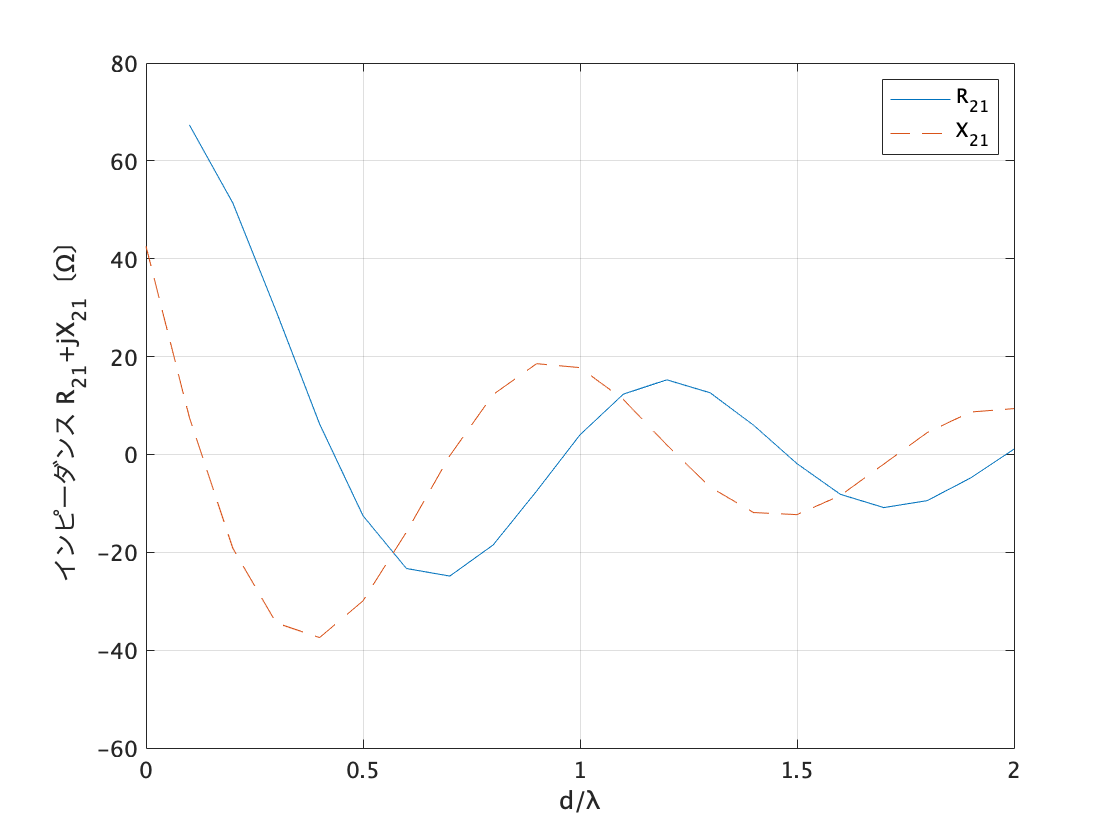
\includegraphics[scale=0.27]{week9_2.png}
  \caption{半波長ダイポールアンテナ間の相互インピーダンス}\label{fig:図2}
\end{figure}
 \\

\begin{lstlisting}[caption=ソースコード,label=1]
  figure 

  lamda = 1;

  k = 2*pi / lamda;
  
  %間隔dが、0から2λまでを0.1λずつ計算
  x = 0:0.1:2;
  
  %相互インピーダンスの実部
  y = 30 * (2*cosint(k*x) - cosint(k * (sqrt(x.^2 + (lamda^2 / 4) )+ (lamda/2)) ) - cosint(k * (sqrt(x.^2 + (lamda^2 / 4)) - (lamda/2))));
  
  %相互インピーダンスの虚部
  y2 = 30 * (-2*sinint(k * x) + sinint(k * ( sqrt(x.^2 + (lamda^2/4) )+ (lamda/2)) ) + sinint(k * (sqrt(x.^2 + (lamda^2 / 4)) - (lamda/2))));
  
  plot(x,y,'-',x,y2,'--')
  
  %xとyの範囲を設定
  xlim([0 2])
  ylim([-60 80])
  
  xticks([0 0.5 1 1.5 2])
  
  grid on
  
  xlabel('d/λ')
  ylabel('インピーダンス R_{21}+jX_{21}〔Ω〕')
  
  legend('R_{21}','X_{21}');
  
    
  \end{lstlisting}


\end{document}
